\documentclass[]{interact}

% AUTHOR
\usepackage{bm}
\usepackage{graphicx}
% \usepackage[none]{hyphenat}
\usepackage{mathtools}
\usepackage{multirow}
\usepackage{nth}
\usepackage[group-separator={,}]{siunitx}
% \usepackage{subcaption}
\graphicspath{{graphics/}}


% PUBLISHER
\usepackage{epstopdf}% To incorporate .eps illustrations using PDFLaTeX, etc.
\usepackage[caption=false]{subfig}% Support for small, `sub' figures and tables
%\usepackage[nolists,tablesfirst]{endfloat}% To `separate' figures and tables from text if required
\usepackage[doublespacing]{setspace}% To produce a `double spaced' document if required
\setlength\parindent{24pt}% To increase paragraph indentation when line spacing is doubled
% \usepackage[longnamesfirst,sort]{natbib}% Citation support using natbib.sty
% \bibpunct[, ]{(}{)}{;}{a}{,}{,}% Citation support using natbib.sty
% \renewcommand\bibfont{\fontsize{10}{12}\selectfont}% To set the list of references in 10 point font using natbib.sty
\usepackage[natbibapa,nodoi]{apacite}% Citation support using apacite.sty. Commands using natbib.sty MUST be deactivated first!
\setlength\bibhang{12pt}% To set the indentation in the list of references using apacite.sty. Commands using natbib.sty MUST be deactivated first!
\renewcommand\bibliographytypesize{\fontsize{10}{12}\selectfont}% To set the list of references in 10 point font using apacite.sty. Commands using natbib.sty MUST be deactivated first!

\theoremstyle{plain}% Theorem-like structures provided by amsthm.sty
\newtheorem{theorem}{Theorem}[section]
\newtheorem{lemma}[theorem]{Lemma}
\newtheorem{corollary}[theorem]{Corollary}
\newtheorem{proposition}[theorem]{Proposition}
\theoremstyle{definition}
\newtheorem{definition}[theorem]{Definition}
\newtheorem{example}[theorem]{Example}
\theoremstyle{remark}
\newtheorem{remark}{Remark}
\newtheorem{notation}{Notation}

% AUTHOR
\bibliographystyle{apacite}

\begin{document}

\articletype{DRAFT}% Specify the article type or omit as appropriate

\title{Spatial demographics with regression kriging: mapping and interpreting social factors of vulnerability to disaster in the Philippines}

% \author{
% \name{C.~M. Armstrong\textsuperscript{a}\thanks{CONTACT C.~M. Armstrong. Email: chandler.m.armstrong@usace.army.mil}, Marina Reilly-Collette\textsuperscript{b}, and Marissa Torres\textsuperscript{b}}
% \affil{\textsuperscript{a}ERDC-CERL, 2902 Newmark Dr, Champaign, IL 61826, USA; \textsuperscript{b}ERDC-CRREL, 72 Lyme Rd, Hanover, NH 03755, USA}
% }

\maketitle

% types of boundaries: geographic, administrative, cultural
\begin{abstract}
  Spatial demographic data is the defining aspect of population geography and a necessary component for decision support.  Spatial analysis often demand specialized methodology, and the physical size of spatial demographic data and the many different needs of its users have left it difficult to develop generalized methods and best practices for this data.  The following discusses interpretation of spatial demographic data and reviews two methods that underlie most techniques for downscaling this data: area-to-point regression kriging and regression weighted dasymetric mapping.  Both methods are ideal for demographic data because both allow modeling with a combination of geographic and demographic factors; an important feature for demographic data with extra-spatial influences.  Both methods can also be used for spatial extrapolation.  After reviewing methods the article uses regression kriging to map a social vulnerability index in the Philippines.  The result is a coherent downscaling of social vulnerability to a one kilometer regular grid that facilitates visualization and combination of multiple spatially-explicit data sets.  The paper concludes with a discussion of concerns that arise when fitting a spatial model using census data from one nation and applying that model to make inferences within the borders of another nation.
\end{abstract}

% mckenzie 1999 for spatial regression examples
% areal interpolation (see for example \citep{montero10, montero11}) or dasymetric mapping (see for example \citep{mennis03, bentley13}.)

% \newpage
\begin{keywords}
  regression kriging; dasymetric mapping; change of support problem; spatial demographics; population geography
\end{keywords}


Maps of the human population are essential for demographic spatial analysis or to support decision-making with spatial components or consequences.  The simplest population maps are based upon demographic data that is aggregated to predetermined boundaries.  These are the {\em choropleth} maps, and for many decades they have been an essential tool of human geography.  The drawback of choropleth maps is that the boundaries are often arbitrary and aggregations within the boundaries may not accurately reflect demographic realities.  Unequal spatial sizes between bounded areas can also produce a visual bias where viewers perceive larger areas as more important.  The problem of arbitrary boundaries is a very generic one, and known as the {\em modifiable areal unit problem} (MAUP).

The MAUP bears important statistical consequences as well.  Openshaw and Taylor \cite{openshaw79} demonstrated that, given the privilege to arbitrarily choose aggregations of counties in Iowa, they could manipulate the correlation between republican voting and proportion of elderly people in a county to between nearly $-1$ and $1$.  Sometimes data is aggregated at a relatively fine scale of semi-regular enumerative boundaries--e.g. census blocks--and such data may avoid some problems of the MAUP.  Another problem, however, is that spatial aggregations are incompatible with any data source not using the same aggregation boundaries.  These two problems, the first of arbitrarily aggregated data and the second of incompatible aggregation boundaries, are both manifestations of a specialized variant of the MAUP known as the {\em change of support problem} (COSP) \citep{cressie96, gelfand01}.  Dasymetric mapping and kriging, which the following article will compare, are methods for solving this problem.

Combining data with different spatial supports is a non-trivial but common problem that occurs when at least one of multiple data sets is associated with a set of polygon features.  Regression weighted dasymetric mapping (RWDM) solves the COSP by downscaling data from a set of source polygons to target polygons or points, based upon statistical correlations between source and target features.  Regression kriging (RK) also uses a regression model to estimate correlations between source and target features, but additionally specifies a spatial autocorrelation model that attempts to explain the residual error of the regression  model as a function of spatial autocorrelation.  The na\"{i}ve method for fitting an autocorrelation function to polygons is to collapse them to their centroids, but this simplification ignores the different sizes and shapes of the polygons.  Methods to accommodate area-to-area/point (A2A/P) spatial autocorrelation also exist, and will be briefly explained in this article.

The estimated quantities of mapped demographic data are typically expected values or probabilities, and not a physical measurement in space.  Nevertheless, spatial population data represent an environmental reality and often can be linked to a real spatial quantity.  For example, a map of the risk of childhood leukemia suggests underlying environmental causes that have a physical spatial reality.  The presence of carcinogens in the environment contribute to an increased rate of childhood leukemia in an area of space, for example, and within this space induce spatial autocorrelation among incidences of the cancer.  An alternative analysis could map concentrations of carcinogens--e.g. concentrations of heavy metals in soil samples.  The two variables, risk of childhood leukemia and concentration of heavy metals, both could be down scaled to an arbitrary spatial support, even to a single point.  Only heavy metals, however, are observable in a single sample.  Risk cannot be directly observed, it is instead estimated from multiple observations and hence is already an aggregate value.  This distinction may be the most important for understanding spatial demographic data.

Survey data is georeferenced to administrative or enumeration boundaries for purposes of convenience, privacy, and anonymity.  Downscaling procedures for demographic data, both dasymetric and kriging, estimate rates or probability densities over areas of space, and could place spatial limitations on demographic attributes that narrow down the identities of people living in an area.  The U.S. Census Bureau has found that georeferenced aggregated tabular data provides means to reconstruct real individuals in the microdata \citep{abowd18, abowd19}.  The conclusion discusses complications that spatial demographic downscaling may pose for privacy of survey data, and additional concerns regarding use of personal data.

The goal of this article is to demonstrate a spatial demographic model in a typical application for the purposes of discussing benefits, difficulties, and caveats of these models in such applications.  The discussion assumes familiarity with linear regression and its underlying linear algebra, but requires no knowledge of spatial modeling.  The first section examines the elements of spatial demographic model design, and reviews the history, applications, and interpretations of spatially explicit demographic data.  The second section outlines the options available for fitting both RWDM and RK models and the criteria for selecting from among them.  The third section demonstrates an RK model in an application of downscaling demographic data for the purpose of visualization.  For this application, the model will downscale a social vulnerability index (SVI) from the municipalities where it is aggregated to a grid of roughly one square kilometers.  The conclusion summarizes the article, highlights the benefits of down scaled demographic data, and touches upon technical and ethical concerns that users should be aware of when applying spatial models for demographic mapping.


\section{Spatial demographic data and models}

In any discipline where they might be useful, demographic maps have almost certainly been utilized.  Geodemography is a practice oriented science of classifying spatial areas of population, often applied in business and public policy (see \citep{acorn} for an example), but also with a parallel academic research arm \citep{oacug, pwnation, singleton14}.  Medical geography create maps of demographic data to help identify and clarify spatial relationships between human medical health and the environment \citep{brown09}.  Population geography is a subfield of human geography that specializes in generating maps of human population by demographic attributes \citep{bailey05}.  Certainly countless other examples exist from the social, political, medical, and economic sciences.  Nonetheless, whereas classical statistics are ubiquitous across social sciences, geospatial statistics remain a specialty technique.

One reason classical statistics may enjoy popularity is because it offers a generalized yet simple framework, and importantly is computationally efficient; ordinary least squares (OLS) offers a computational complexity of $O(C^2N)$ versus kriging complexity of $O(N^3)$, required to invert the $n \times n$ kriging covariance matrix.  RWDM, which essentially is simple linear regression, can be performed with most contemporary personal computers, whereas RK consumes considerable computing resources and may demand high-performance hardware and software.  This stark difference in physical limitations may require that data management and analyses of geospatial data be shifted from personal to cloud computer resources.  The lack of a simple and generalized kriging framework, on par with the usability of those available for classical statistics, is also a serious obstacle that receives insufficient attention.

The following section discusses spatial demographic data and provides definitional equations.  The first subsection briefly examines types of demographic data and their modeling implications.  The second takes a closer look at the COSP.  The third and final subsection compares the equations for RWDM and RK, and discusses their differences and similarities.  These subsections will discuss properties of the data and models that will be referenced when this article analyzes a RK model for an application of mapping social vulnerability.


\subsection{Types of demographic data}
% lark04

For modeling purposes, demographic data come in two types: continuous and discrete.  Continuous data exists on the real number line, and thanks to statistical innovations like the central limit theorem, most continuous data can be modeled using linear models and the normal distribution.  Discrete variables may take only certain values; examples include binary data, proportions, and counts.  Discrete data are not normally distributed but instead follow the binomial, multinomial, or Poisson distributions.  Conventional regression and kriging models assume normally distributed data, and require modifications to work appropriately with discrete data.  Regression models fit to variables with two or more discrete classes are known as binomial or multinomial respectively.  Indicator kriging is a methodology for fitting kriging models to discretized data, and Goovaerts \cite{goovaerts10} recommends variations of indicator kriging for binomial and ordinal spatial demographic data.

RWDM is essentially a regression model fit to georeferenced data.  OLS is appropriate for continuous data, and discrete models are available within the framework of generalized linear modeling (GzLM).  Using GzLM, one supplies a link function and distribution.  The link function linearizes the data, and the distribution describes the distribution of the errors in a model of the data.  GzLM fits a model to the data using iteratively reweighted least squares to maximize the likelihood for the given distribution \citep{nelder72}.  OLS is a form of GzLM, with an identity link and normally distributed errors.  % display an equation with link function?

% mention disjunctive kriging?
Extending kriging models is more difficult, and a generalized framework for both linear and non-linear models doesn't seem to exist for kriging.  Kriging may be employed for discrete data, but it may not correctly model the variance properties \citep{goovaerts10}.  Goovaerts addressed the issue of kriging small samples of Poisson distributed data by adding a Poisson variance term to the kriging equations that represents the intrinsic unreliability of small counts \citep{goovaerts06}.  A like method is applicable to binomial data, replacing the Poisson-distributed variance with binomial variance \citep{goovaerts04, goovaerts09}.  Indicator  kriging (IK) is another framework for discrete data that was designed to analyze discretizations of continuous data \citep{journel83}.  Outliers are pathological for kriging models, but may be removed by discretizing the data as either above or below a threshold.  Multiple discrete data sets can be generated for different threshold values, and all data sets cokriged--a multivariate kriging, similar to multivariate regression.  Binomial cokriging is a similar method designed for kriging proportions \citep{lajaunie91, oliver98}, where unobserved continuously varying probability of incidence at some point in space $x(s_0)$ is estimated along with observed aggregated proportions.

Specialized extensions of kriging notwithstanding, the performance of basic kriging models with discrete data is often sufficient, and at times more stable than more complex models \citep{oliver98}.  Kriging of binomial data, however, may yield results outside the range of $[0, 1]$.  This occurs where samples of data are tightly clustered.  Kriging declusters data by distributing weight equally around the clustered points, and the optimization often assigns negative weights to some points of a cluster to balance large positive weights assigned to others.  Negative weights can yield results outside observed data ranges, and in general disturb performance of a kriging model \citep{duetsch96}.  One can avoid negative weights by using spatial variance-over-distance functions, the so-called variogram, that increase quickly.  Using a Gaussian cumulative distribution curve for a variogram function will overweight nearby samples due to the flatness of the curve close the origin: the curve models nearby data points as too similar and overweights nearby points while underweighting outlying data.  Overweighting some points of a cluster requires that some other members receive negative weights to balance out the distribution of weights.  This is sometimes called the {\em screen effect}, as negative weights are compensating for overweighting of nearby data that screen out distant data.  Variogram functions less prone to negative weights include the exponential and spherical functions, which both increase quickly at the origin.  Gaussian curves are optimal for truly normally distributed data--e.g. distribution of gas concentrations in a body of air--but in general spatial data is not normally distributed.


\subsection{Change of support problem}

The COSP refers to inference of values at points or areas that are different from those where values have been observed \citep{gelfand01}.  In cases where observations are available only as an aggregation to an area, and where the goal is to estimate new values over unobserved areas, the problem is more generally referred to as the MAUP \citep{cressie96}.  % see gelfand for COSP citations, track down mugglin for more methods on areal weighting.

Dasymetric mapping was developed, essentially, to solve the COSP for population data.  Generically, dasymetric maps downscale spatial data from a larger source zone to intersecting target zones using ancillary attributes of the target zones to determine population distribution.  Regardless of its simplicity, the method consistently performs well at this task \citep{eicher01, holt11, barrozo16, amos17}.  Dasymetric mapping does not directly model spatial autocorrelation, nor can it spatially interpolate data; it depends entirely upon relationships in {\em feature space}--the ancillary data--rather than in geographical space.

Kriging was developed to model and estimate spatial distribution of natural resources.  The notable feature of kriging is that it models spatial autocorrelation of the data, and not the actual data values.  In contradistinction to dasymetric mapping, kriging was originally designed to aggregate data--so called block-kriging \citep{cressie90, matheron63}.  Conventionally, kriging analyzes samples of point data in order to estimate a complete spatial distribution for the purpose of summarizing the resources available over an area of space.  With its original design scope, kriging required modifications to estimate a spatial distribution from data aggregated in polygons.  The solution is A2A/P kriging \citep{krivoruchko11, kyriakidis04}.

The basic technique of A2A/P kriging is to discretize the polygons into a series of regular points, and estimate the spatial autocorrelation between any two polygons as the average correlation of their discretizing points \citep{kyriakidis04}; similarly correlation between points and polygons is the average of correlation between the point and discretizing points of the polygon.  A2A/P kriging is a type of binomial cokriging, mentioned in the previous section, where the discretized polygon data is cokriged with target discretization points from other polygons or a regular grid where one wishes to interpolate data, i.e. the target support.  This whole procedure works because, as the next section will discuss, kriging models only variance as a function of distance between points, and does not need access to underlying data.  The kriging model is simply an autocorrelation model that describes how {\em best}--as in best linear unbiased estimate (BLUE)--to interpolate observed data to unobserved supports.
% ESRI tested area-to-area kriging for applications to demographic data and found the results to generally be within acceptable limits of accuracy \citep{carson13}.  Amos et al \citep{amos17} compared area-to-area and area-to-point kriging with dasymetric mapping--which we will dicuss shortly--for the purpose of distributing census data into voting precints that are split by a census block; their results found that dasymetric mapping was superior for this application, and that kriging estimates often fell outside of recommended error bounds.

In regards to downscaling of demographic data, the issue of binomial data and COSP often are the same.  Even where raw point data is available, demographic data is often aggregated to a boundary where it can be converted to a proportion.  Methods like binomial cokriging reflect this link between the COSP and binomial data.


\subsection{Regression kriging and regression weighted dasymetric mapping}

RK and RWDM may be compared roughly in terms of the assumptions each makes about space.  Kriging assumes that the data varies continuously over space and is spatially autocorrelated, such that a set of closely clustered locations are more similar to each other than a set of widely scattered locations.  Dasymetric mapping ignores spatial factors like shape, size, and distance, and instead assumes that spatial relationships can be described entirely by the values of ancillary data sources.  The accuracy of either method depends, essentially, upon an ability to identify spatially homogeneous areas \citep{maantay07, maantay08}.  Kriging and RWDM exemplify this difference, in that the former models only spatial autocorrelation, and the latter models only correlations with the ancillary data.  RK combines both methods; a topic this section will presently examine.
% demographic characteristics can change sharply at arbitrary geographic boundaries \citep{schelling71}.
% reibel also points out that interpolation methods make an assumption of smooth variance that is often unsupportable where administrative and political boundaries coincide with real geographic boundaries.
% gooaverts, gotway & young, kyriakidis, amos, carson for discussion and evaluation of kriging for demographic data
% see amos page 392 for discussion and citations on the problems of interpolation and kriging applied to population data.

The kriging interpretation of spatial data is somewhat fraught for demographics, where all data is attached to discrete objects--people--and cannot usefully be viewed as realizations of a smooth and continuous random field (see \citep{cova02, kjenstad06} for discussion of the distinction between spatial fields and objects.)  Nonetheless, choropleth maps represent a set of expectations for a variable, each bounded and constant over an area of space, and it's quite natural to imagine how this could be converted to a smoothly varying function over space.  Schmid and Maccannell\cite{schmid55} and later Tobler \cite{tobler79} analyzed the production of contour maps from choropleth maps and control points of population density data.  Kriging accomplishes the same task within a framework of analysis of spatial autocorrelation.

% Dasymetric mapping methods can be broadly categorized into three types: area weighted, homogenously weighted, and regression weighted \citep{reibel07}.  All three methods share a common goal of downscaling data from larger source zones to smaller target zones.  Area weighted is the simplest of the three, and simply reportions data between a source and target areas based on the respective size of each target area within the source area (see \citep{goodchild80} for an example).  Homogenous weighting searches for source zones that are completely covered by each category available in the ancillary data, and uses these zones to estimate the population density for that given category (see for example \citep{eicher01, mennis03}).  Regression weighting regresses population counts from source zones upon the area of each ancillary category within the source zone to obtain population density weights (examples are \citep{flowerdew89, flowerdew92, reibel07}.)  By fitting ancillary category indicators to population counts using a Poisson distribution, the coefficients for each category may be interpreted as the  population density of that particular category \citep{reibel07}.  Regression weighting might be the most sophisticated of the three dasymetric methods, but with modern software it is simple to apply and interpret, and avails any analysis of a vast array of regression methods.

The data for both RK and RWDM is similar, consisting of a matrix of $m$ predictors $X$ and a vector of $n$ observations $\bm{y}$ thought to be dependent upon $X$, where typically $m \ll n$.  Kriging models covariance between data points of $\bm{y}$, assuming these are realizations of random variables with a multivariate Gaussian distribution, and is generally equivalent to a Gaussian process (GP) regression model \citep{rasmussen06}.  RWDM analyzes covariance between the columns of $X$ and $\bm{y}$ using OLS or GzLM.  In addition to data values, kriging requires spatial coordinates of the data, usually written $\bm{y}=\{y(s_i), ..., y(s_n)\}=y(S)$ and $X=\{\bm{x}(s_i), ..., \bm{x}(s_n)\}=X(S)$ to emphasize that the data is generated by a function with a spatial coordinate.  The values of $\bm{y}$ are measurements at the locations of $S$--e.g. a volume of mineral, inches of rainfall, or height of a plant.  The matrix $X$ is a data set of co-located measurements that represent independent variables.  Both methods begin with an input of $n$ cases $\{(y(s_i), \bm{x}(s_i)), ..., (y(s_n), \bm{x}(s_n))\}$ and derive a vector of weights for estimating values at unobserved location $s_0$.

Regression weights, or regression coefficients, weight the impact of variable $x_j(s_0)$ on the estimate of $y_0$ at location $s_0$:

\[\hat{y}(s_0) = \sum_{j=0}^m \beta_j x_j(s_0); \; x_0(s_0) \equiv 1\]

The constant term $x_0$ is set to $1$.  Kriging weights are similar, but rather than weight the effects of variables they instead weight the influence of nearby data points:

\[\hat{y}(s_0) = \sum_{i=1}^n \lambda_i y(s_i)\] % ; \; \sum_{i=1}^n \lambda_i \equiv 1\]
% Where the weights are constrained to sum to $1$ to guarantee unbiasedness, do to the fact that $\hat{y}=y$ for any $s$.

The mathematical notation emphasizes that values of $\bm{y}$ and $X$ are indexed to spatial locations by writing them as functions of location: $y(s_0)$ and $\bm{x}(s_0)$.  We'll see that RWDM doesn't analyze location or spatial arrangement, and is based only on the values generated by those functions.  In contradistinction most forms of kriging don't analyze ancillary data, and are based only on analysis of spatial arrangement.  RK combines the two methods to analyze both ancillary data and spatial arrangement.  We begin by describing the algebra and assumptions of regression that underlay RWDM; RK will use these same regression methods within the kriging framework, and by introducing the regression assumptions first we can see how these assumptions manifest in the kriging framework.


\subsubsection{Regression weighted dasymetric mapping}
% for a fuller discussion on the assumptions, diagnostics, and variants of linear modeling, see \citep{nelder72, mardia80, gelman06}.

OLS finds regression weights that minimize the sum of squared errors:

\[\sum_1^n (y_n - X \bm{\beta})^2 = \sum_1^n \epsilon_{n}^2 \]

The first column of the matrix $X$ are ones for the constant term, the other columns are the data.  The weights $\bm{\beta}$ that minimize $\sum_1^n \epsilon_{n}^2$ are a function of the covariance of the data:

\[X^T X \bm{\beta} = X^T \bm{y} \]

% is X^ty a moment matrix?
Where $X^TX$ and $X^T\bm{y}$ are the moment matrices corresponding to the second moments of $X$ and $X^T\bm{y}$ with $\dim{X^TX}=m \times m$ and $\dim{X^T\bm{y}}=m \times 1$.  The matrix $X^T X \bm{\beta}$ is a system of equations, solving by inverting results in the familiar OLS equation:

\begin{equation} \label{eq:ols}
  \bm{\beta} = (X^T X)^{-1} X^T \bm{y}
\end{equation}

The best estimate for an unknown $y_0$ given input data $\bm{x}_0$ is

\[\hat{y}_0 = \bm{x}_{0}^T \bm{\beta}\]

with variance equal to

\[\hat{\bm{\epsilon}}=\bm{y}-\bm{\hat{y}}\]
\[\sigma^2=\frac{\hat{\bm{\epsilon}}^T\hat{\bm{\epsilon}}}{n-m}\]

OLS imposes a few important assumptions.  The first is that $E[\bm{\epsilon} | X] = 0$, a result of the fact that OLS minimizes the sum of $\bm{\epsilon}^2$.  The first assumption is the most important, it is what guarantees that the model is unbiased and free of confounding effects, and violating the first assumption will invalidate the model.  The second assumption is that no variables are linearly dependent, and is required to solve the system of equations (i.e. invert) $X^TX$.  A linearly dependent variable is also collinear, hence all but one of the collinear variables may be removed to obtain the assumption of linear dependence.  The third is that $\bm{\epsilon}^2$ has the same conditional variance $\sigma^2$ for all observations--i.e. homoscedasticity--and that $\bm{\epsilon}^2$ is uncorrelated between observations, these two criteria together form the assumption of spherical errors.  If the assumption of spherical errors does not obtain, the OLS estimates are still valid but the model is less efficient.  This third assumption, in fact, is the essential difference between OLS and kriging methods: kriging relaxes the third assumption by modeling spatial autocorrelation between observations.
% assumptions are strict exogeneity, linear independence of $\bm{X}$, homoscedasticity, no autorcorrelation, normally distributed errors, and independently and identically distributed observations.

RWDM does not, in general, preserve the original volumes of the source zone data used to estimate values in the target zones.  This property is sometimes referenced as coherence or exactitude, and it is an attractive property of kriging.  Because RWDM lacks this property, users should usually rescale the estimates so that, when summing across target zones within a source zone, the sums equal the original source zone data.  The equation to accomplish this is:

\[\hat{y}^{'}_{i\cdot} = \hat{y}_{i\cdot} \frac{y_i}{\sum_{j=1}^{n_i} \hat{y}_{ij}}\]

where $\hat{y}^{'}_{i\cdot}$ is a rescaled estimate within source zone $i$, $\hat{y}_{i\cdot}$ is the raw estimate, $y_i$ is the observed value of source zone $i$, $n_i$ is the number of target zones that intersect source zone $i$, and $\sum_{j=1}^{n_i} \hat{y}_{ij}$ sums over all $j$ raw estimates in source zone $i$.


\subsubsection{Regression kriging} \label{sec:rk}

RK analyzes data in two steps.  The first step is essentially identical the RWDM described in the previous section.  Rather than keep the fitted values, however, RK will map the residuals.

\[\hat{\bm{\epsilon}} = \hat{\bm{y}} - \bm{y}\]

The second step of RK interpolates the residuals using kriging, with the ultimate effect of allowing the mean of the kriging system to vary based upon the RWDM model output.  Simple (SK) and ordinary kriging (OK) are the two most basic forms of kriging, and both assume the data is generated by an intrinsically stationary process with a constant but known (SK) or unknown (OK) mean over a sample area.  Residuals by definition have mean $0$, hence RK uses SK to interpolate the residuals over an area.  All forms of kriging assume that the observed data $\bm{y}=\{y(s_i) | i=1, ..., n\}$ is a single sample from a multivariate Gaussian process at locations $S=\{s_i | i=1, ..., n\}$.

SK is, unsurprisingly, simpler than OK.  List~\ref{lst:kriging} gives the data generating equations modeled by SK, OK, and RK--for comparison purposes.  Although the only difference between SK and OK here is the mean parameter $\mu$, this has important consequences for the objective functions that OK must minimize, and for the properties of the resulting model.  OK assumes only intrinsic stationarity, and models a constant local mean $\mu_{x_0}$.  SK, on the other hand, assumes a known mean and thus a globally stationary constant $\mu$ that can be shifted to zero without loss of generality.  Lacking a prior known mean, OK also has no way to compute a covariance function and instead uses a variogram to model covariance.  Under most circumstances all major properties of covariance functions carry over to variograms \citep{gneiting00, wackernagel03a}.  % empirical semivariogram
A final important difference is that OK uses a Lagrangian multiplier to constrain the kriging weights to sum to one.  The role of the Lagrangian in OK equations can be difficult to visualize geometrically.  In this case, the Lagrangian can be understood as constraining the optimization of the OK equations to a point in the $\dim{\bm{\lambda}} = n$ dimensional space where the kriging weights sum to one.  The kriging weights are similar to those for a weighted mean, and if they do not sum to one then some values will be over or underweighted yielding a result that is biased from the mean.  See Wackernagel \cite{wackernagel03a} chapter 11 for a formal derivation of the OK system of equations using a Lagrangian multiplier.% This necessity arises because the expected value $\mu(x_i)$ of the observed locations and the estimated location should be equal: Hence, the weights must sum to one to ensure unbiasedness.
% Where $\sigma_n$ is the so-called {\em nugget} effect that models discontinuity at the origin due to measurement error or variation below the spatial scale available in the data.  In geospatial sciences, the hyperparameter $\sigma_f$ is usually the {\em sill}, or maximum variance.  If a variogram is bounded--i.e. approaches the sill or asymptote--then it shares all major properties of covariance functions, which are necessarily bounded to be positive semidefinite.  Not all variograms are bounded, however, for example a variogram based upon a linear covariance function is unbounded.  For this reason, geospatial statistics generally limit variograms to covariance functions that yield bounded variograms, in particular the spherical and exponential family of covariance functions \citep{}.


\begin{enumerate}\label{lst:kriging}
\item simple: $y_i = e_i$
\item ordinary: $y_i = \mu + e_i$
\item regression: $y_i = x_{i}^T \beta + e_i$
\end{enumerate}

% \begin{description} \label{lst:kriging}
% \item[dasymetric] distribute data between zones based on weights over features:\\
%   $y_n = \sum_1^m x_{nm} \beta_m; \; {1, \dots, n}$
% \item[kriging] distribute data between zones based on weights over functions:\\
%   $y_n = \sum_1^m y_m \lambda_{nm}; \; {1, \dots, n}$
% \item[regression kriging] kriging with varying mean:\\
%   $y_n = \sum_1^m (E[y_m]-y_m) \lambda_{nm}; \; {1, \dots, n}$
% \end{description}

The regression kriging equation in table~\ref{lst:kriging} is oversimplified for comparison purposes; the complete RK equation is:

\begin{equation} \label{eq:rk}
  \hat{y}(s_i) = \bm{x}(s_i)^T \bm{\beta} + \bm{\lambda}_i (\bm{x}(s_i)^T \bm{\beta} - \bm{y}(s_i))
\end{equation}

The equations in table~\ref{lst:kriging} omit the spatial indexes, and collapse the second term in the RK equation to $e_i$: the interpolated residual.  RK is further subdivided based upon how the $\beta$ parameters are obtained.  If $\bm{\beta}$ is derived external to the RK model, and provided as input, this method is conventionally referred to as {\em universal kriging} (UK) \citep{pebesma06, hengl07a}.  If on the other hand the $\bm{\beta}$ parameters are fit along with the coordinates of the data locations, as part of the kriging equations, then this method is usually referred to as {\em kriging with external drift} (KED).  The two methods yield identical results in most cases, however UK, because it accepts externally derived $\bm{\beta}$ parameters, can be used to extrapolate data to new locations.  The ability to fit a RK model in one location and apply it in another raises important technical and ethical issues that will be revisited for a discussion within the concluding section.  For derivations of SK and OK see \citep{wackernagel03a} or \citep{gotway97}, and for a comparison of RK, UK, and KED see \citep{hengl07a} or \citep{wackernagel03a}.  SK is equivalent to GP regression, as described in \citep{rasmussen06}.

From the data SK builds a matrix, a row vector, and scalar:

\[V=
  \begin{bmatrix}
    c(s_1, s_1) & \cdots & c(s_1, s_n) \\
    \vdots      & \ddots & \vdots \\
    c(s_n, s_1) & \cdots & c(s_n, s_n)
  \end{bmatrix}
\]

\[\bm{v}_0=[c(s_0, s_1), \cdots, c(s_0, s_n)]\]

\[v(s_0)=c(s_0, s_0)\]

The function $c$ is the covariance function--or kernel, in GP terminology.  Kriging assumes both first and second order stationarity--so that all data points share $V$ and $v(s_0)$.  The matrix $V$ is the $n \times n$ covariance matrix for all observations.  The vector $\bm{v}_0$ is the $1 \times n$ row vector of variances between the coordinates $s_0$ and those in $S$, this vector is subscripted to emphasize that it is recomputed for each $s_0$.  The scalar $v(s_0)$ is the maximum variance $\sigma_{y}$ of $y_0$, and because we assume a stationary second moment it also is the maximum variance of all the measurements; therefore it is equal to the values on the diagonal of $V$.  Although the covariances of $V$ are functions only of the distance values in $S$, the kernel $c$ has a number of free {\em hyperparamters} (e.g. $\sigma_y$) that must be estimated from $\bm{y}$.  Indeed, the assumptions of constant mean and variance is equivalent to assuming that the data generation process is sufficiently homogeneous over the area of interest to allow for mean and variance to be estimated from the data; this is what allow the hyperparameters to be estimated from empirical data and build the matrix $V$.  As mentioned previously, OK doesn't assume a known mean and models $V$ using a (semi)variogram rather than a covariance; this distinction is academic for most, however, and most practitioners can treat these two things identically.  It's critical to note that, other than hyperparameters, the data in $\bm{y}$ isn't used to compute covariance matrix $V$ and friends; these constructs represent only the spatial correlation in $S$.

% https://stats.stackexchange.com/questions/77483/kriging-without-covariance
% The semivariogram $\gamma$ is related to the covariance function $k$ in~\ref{eq:vgm2cov}.

The kriging weights are derived by solving the system of equations:

\[V \bm{\lambda}_0 = \bm{v}_0 \]
\[ \bm{\lambda}_0 = \bm{v}_0 V^{-1} \]

The probability of a particular estimate for $y_0$ is given by:

\begin{equation} \label{eq:posterior}
  y_0 | \bm{y} \sim N(\bm{v}_0 V^{-1} \bm{y}, \, v(s_0)-\bm{v}_0^T V^{-1} \bm{v}_0^T)
\end{equation}

% I mention unbiasedness, but not minimum variance...
where the best estimate $\hat{y}_0$ is the mean parameter of the normal distribution $N$ (the first parameter.)  Notice that the kriging weights, $\bm{\lambda}_0=\bm{v}_0 V^{-1}$, depend upon the location $s_0$ via $\bm{v}_0$ and weight the impact of $\bm{y}$ upon the estimate $\hat{y}(s_0)$.  The weights are subscripted to emphasize that they are computed for each $s_0$.  A consequence of the assumption of a constant mean over the sample area is that $E[\hat{y}_0 - y_0]=0$, or that the estimate is unbiased.  Notice also that, as the covariance is stationary (the second parameter of $N$), it too doesn't depend on the values of $\bm{y}$.  The two most important aspects of these equations is 1) the kriging weights only depend on the locations in $S$ and 2) they model covariance between these locations.

The kriging weights $\bm{\lambda}_0$ are similar in function to the regression weights $\bm{\beta}$: $\bm{\beta}$ weights the effect of the variables in $X$ on $y_0$, whereas $\bm{\lambda}_0$ quantify the influence of the observed values in $\bm{y}$ given their distance from the unobserved location $s_0$.  This difference implies another one of importance: the values of $\bm{\beta}$ are the same for any given $\bm{x}(s_0)$, whereas kriging weights depend upon the location $s_0$; kriging fits a regression model for each input point, and must develop the vector $\bm{v}_0$ for each point.  One might say another difference is that OLS weights imply a varying mean, whereas kriging assumes a constant mean; however this comparison is ill-posed.  Kriging allows for varying deviation from the mean, and this property is a better comparison with OLS' varying mean.  Moreover, the constant mean of kriging is more akin to the intercept, or constant, term of an OLS model.  A similarity between both kriging estimates and those provided by OLS are that all estimates are assumed to have the same variance, as dictated by kriging's assumption of second order stationarity, and OLS' homoscedasticity of variance.  This assumption regarding variance for the system of kriging equations should not be confused, however, with the prediction variance of kriging, given by:

\[v(s_0) - \bm{v}_0^T V^{-1} \bm{v}_0\]

The same as the variance parameter of $N$ in the prediction probability given by equation~\ref{eq:posterior}.  Prediction variance of kriging expresses the uncertainty of an estimated value as a function of its distance from observed values.  Homogeneity of variance, on the other hand, refers to the spherical variance of the covariance matrix $V$.

The matrix $V$ and friends are also similar to the moment matrices of OLS.  The comparison between GP and linear regression is usually drawn between GP and Bayesian linear regression (BLR), as BLR is identical to GP with a linear kernel.  BLR also relates to OLS via the equation for the posterior distribution $\textsc{likelihood} \times \textsc{prior}$.  OLS and BLR share identical values for maximum likelihood and as $n$, the number of cases, increases towards infinity the likelihood ``washes out'' the priors, and the estimates of OLS and BLR converge.  What GP does differently is that, whereas BLR analyzes distributions over parameters, GP analyzes distributions over functions \citep{williams97}.  The distinction is clear with a linear kernel $\sigma^2\phi(X)^T\phi(X)$, where $\phi$ is a basis function (possibly identity.)  GP with a linear kernel is BLR with priors over functions.  The matrix form of the linear kernel is quite familiar from the OLS equation $\hat{\bm{\beta}}=(X^TX)^{-1}X^Ty$, from which we may derive the covariance of the weights $\bm{\beta}$ around their true values to be $E[(\hat{\bm{\beta}} - \bm{\beta})(\hat{\bm{\beta}} - \bm{\beta})^T] = \sigma^2(X^TX)^{-1}$, which we can see is identical to the linear kernel (with identity basis).  In essence, GP with a linear kernel would be similar to linear regression that computes moment matrices as $\dim{XX^T}=n \times n$ rather than $\dim{X^TX}=m \times m$.  Kriging rarely uses a linear kernel, however, for which instead conventional kernels include exponential, spherical, Gaussian, and Mat\'{e}rn.

The above brief summary comparison of RK and RWDM is designed to illustrate one important difference.  Kriging is a smoothing model that estimates values at unobserved locations based on distance from observed data and the autocorrelation structure among the observed data.  RWDM is a linear model that estimates values at unobserved locations based on the covariance of the attributes at the unobserved location with the known data, given the covariance structure of the known data.  This is an important distinction for policy and decision makers, where similarity between observed and unobserved locations may depend more upon similarity of their attributes rather than similarity of their spatial location (however, for applications where the estimated data does vary smoothly over the sample area, RK clearly outperforms RWDM \citep{bourennane00}).  RWDM, however, may be simpler to apply in practice since it is basically a general(ized) regression model, and doesn't require the intermediate step of selecting and parameterizing a covariance function.
% kriging can incorporate additional attributes via regression-kriging \citep{hengl07}, also known as universal kriging \citep{wackernagel03}, or kriging with external drift \citep{bourennane00, hudson94}.


\section{Mapping social vulnerability} % and impacts for policy

Solutions to the COSP help researchers to improve visualization of their data and build models that combine data from multiple sources and spatial resolutions.  This final section will demonstrate RK in an application to downscale a social vulnerability index (SVI) from administrative divisions to a regular grid.  This section will review the SVI and its construction, and consider independent predictors for the SVI.  In addition to the SVI factors, the discussion will also analyze how geographical arrangements can be converted into metrics that are predictors of social vulnerability.

SVI is a nebulous and context dependent concept, and important components of a SVI metric may vary depending upon purpose and location.  Many different researchers and organizations have defined an SVI, and this section uses the SVI developed by Ignacio for predicting vulnerability to natural disasters in the Philippines \citep{ignacio15}.  Ignacio obtained census data from Philippines Statistics Authority and computed SVI from neighborhood, or barangay, level data.  The following procedure uses data from IPUMS-International \citep{ipumsi} that is georeferenced to municipalities.  Table~\ref{tab:svi} lists the factors of Ignacio's SVI, and what each represents.  To produce SVI, these factors are combined using principal components analysis (PCA.)  We retain only the first component to represent SVI, although some analyses may retain more.  This SVI value is normally distributed with mean $0$ and standard deviation $1$, where positive values indicate greater than average vulnerability and opposite for negative values.  The average depends upon the input data--an SVI built with Philippines data represents variance around average vulnerability for a Filipino family.

\begin{table}
  \begin{tabular}{l l l}
    \hline
    \bf{variable} & \bf{unit} & \bf{vulnerability concept} \\
    \hline
    \% female & person & gender \\
    \% children & person & age \\
    \% elderly & person & age \\
    \% adults with no secondary degree & person & education \\
    \% with no birth registration & person & social dependence \\
    \% 20-39 year females with no secondary degree & person & education\&gender \\
    \% households with female head & household & gender\&family \\
    \% households with disabled & household & special needs \\
    \% heads of household with no secondary degree & household & education \\
    \% single heads of household & household & family \\
    average size of household & household & family \\
    \% households with no overseas worker & household & social dependence \\
    \% households with poor roofing & dwelling & residence \\
    \% households with poor walling & dwelling & residence \\
    \% households with no tenure & dwelling & social dependence \\
    \% houses over 30 years & dwelling & residence \\
    \% houses needing repair & dwelling & residence \\
    \% houses $< 10m^2$ & dwelling & socioeconomic status \\
    \hline
  \end{tabular}
  \caption{Components of the Social Vulnerability Index} \label{tab:svi}
\end{table}

The unit of analysis of an SVI is the family, however it has limited validity applied to single families, and the values are more usefully aggregated to a geospatial area--so that SVI is a property of a community that encompasses the people, housing, and labour available to a spatial location.  The Philippines SVI data is attached to administrative divisions, to which they can be aggregated and geospatially located.

Along with the SVI, we have a set of geospatial predictors at the target support and will use RK to rescale the SVI data from polygons to this support.  Some of these data are observations of the physical environment, often collected and compiled for years or decades, and available preprocessed and in a format designed for analysis; these could include climatology, landcover, crop \& livestock, human population density, and nighttime lights among others.  There also exist complex data on the human-built environment, including buildings, roads, utilities, and infrastructure.  These latter data facilitate computation of geodemographic metrics reflecting accessibility to social and economic resources.  Pebesma \citep{pebesma06} notes that such metrics are ``cheap'' (quotes in original) because this kind of data is generally freely available--e.g. OpenStreetMap \citep{osm}.  Cheap they may be, it requires lab time and labour to determine, justify, and implement these metrics.  Parsimony demands the metrics be few and simple--which is tragically more difficult than computing masses of random spatial metrics.  The SVI RK model uses only one cheap predictor, but it took years of research to devise and justify: Weiss' accessibility to cities metric \citep{weiss18}, listed in table~\ref{tab:predictors} along with the others used in the model.  Most metrics used in the SVI RK model are not spatial computations or even zonal statistics, but merely observations at a point in space; this also seems to be the case for most spatial models.
% uchida08, linard12, weiss18
% Review of the literature also suggests that, for land use classification, kriging is more often applied {\em post hoc} to existing land use classifications as a means to improve spatial uncertainty quantification (see for example \citep{freeman06, debruin00}.)

\begin{table}
  \begin{tabular}{l p{5cm} l}
    \hline
    \bf{variable} & \bf{source} & \bf{vulnerability relation} \\
    \hline
    urban landcover & \citep{basevue13} & accessibility \\
    agricultural landcover & \citep{basevue13} & socioeconomic status \\
    nighttime lights & \citep{elvidge17} & infrastructure \\
    population density & \citep{landscan} & socioeconomic status \\
    access to cities & \citep{weiss18} & accessibility \\
    \hline
  \end{tabular}
  \caption{Predictors of SVI for RK model} \label{tab:predictors}
\end{table}

The data in table~\ref{tab:predictors} are the predictors to essentially a RWDM model of social vulnerability.  In our case, we will use KED to fit the $\bm{\beta}$ values, but as discussed the results are very similar to UK.  The SVI is a continuous linear value, so it could be fit with a simple OLS model.  The following equation would specify the model.

\[y=\alpha+\beta_1x_{pop}+\beta_2x_{pop}^2+\beta_3x_{urban}+\beta_4x_{ag}+\beta_5x_{travel}+\beta_6x_{lights}\]

The predictor variables are population $x_{pop}$, urban landcover $x_{urban}$, agricultural landcover $x_{ag}$, travel time to nearest city $x_{travel}$, and nighttime lights $x_{lights}$.  The equation is quadratic in population density, to allow for the effect of population density upon SVI to vary with population density.  The kriging step computes the residuals $\bm{x}(s_i)^T \bm{\beta} - y(s_i)$ of the regression model for a regular grid and fits the kriging model to the entire land mass of the Philippines, using the RK method described in section~\ref{sec:rk}.  The computational procedure for fitting the model allows for options to control behavior of the fitting procedure, but which we've skipped here for brevity.  In particular, users of kriging are advised to consider options that force the kriging system to compute covariances using only data within a maximum distance of a target point or only data up to a threshold number of data points.  Both these options limit the size of $V$ and $\bm{v}_0$, which may be a scientifically sensible thing to do, and moreover can allow larger models to be fit on modest hardware.

\begin{figure}
  \centering
  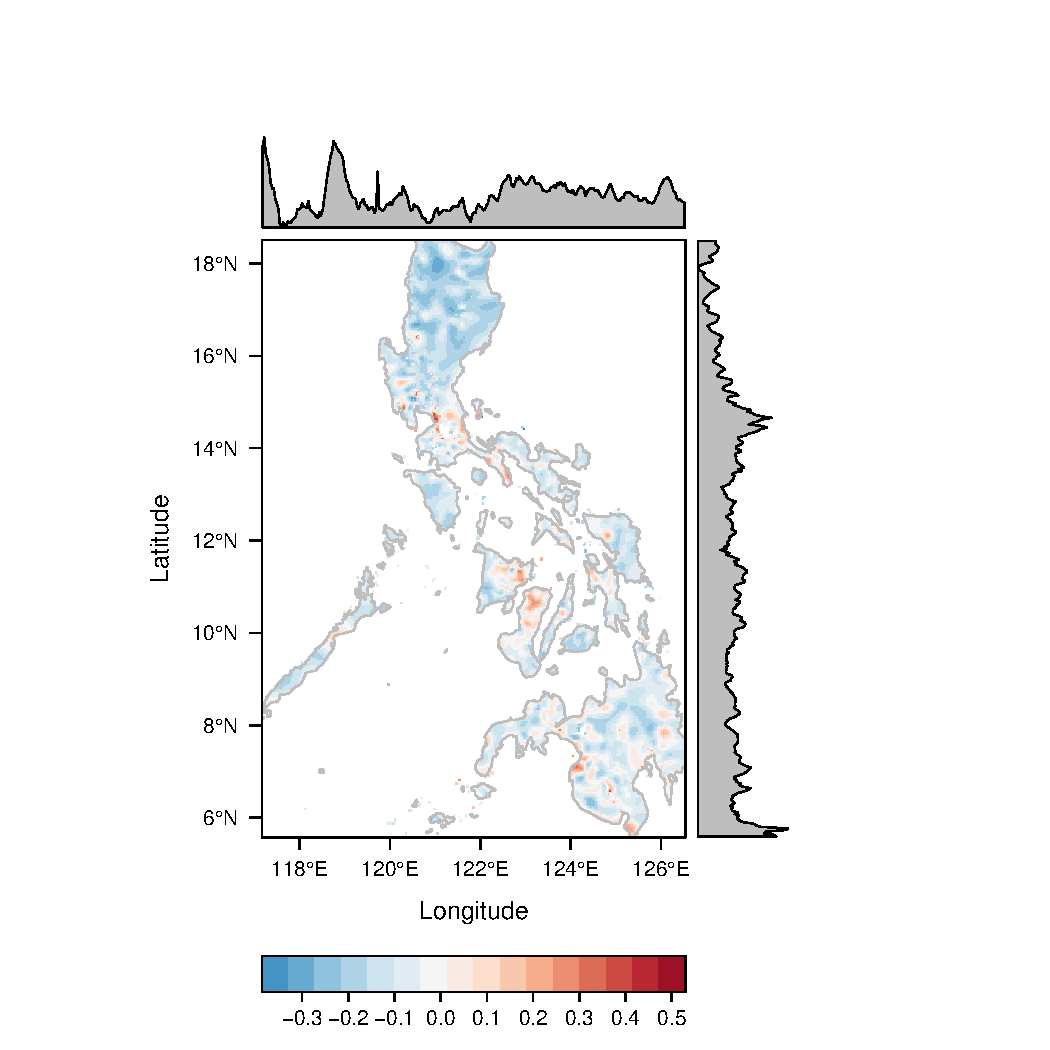
\includegraphics[width=0.8\textheight]{svi.pdf}
  \caption{Social vulnerability, Philippines, 1km scale} \label{fig:svi}
\end{figure}

\begin{figure}
  \centering
  \subfloat[\label{fig:sviNCR}]{
    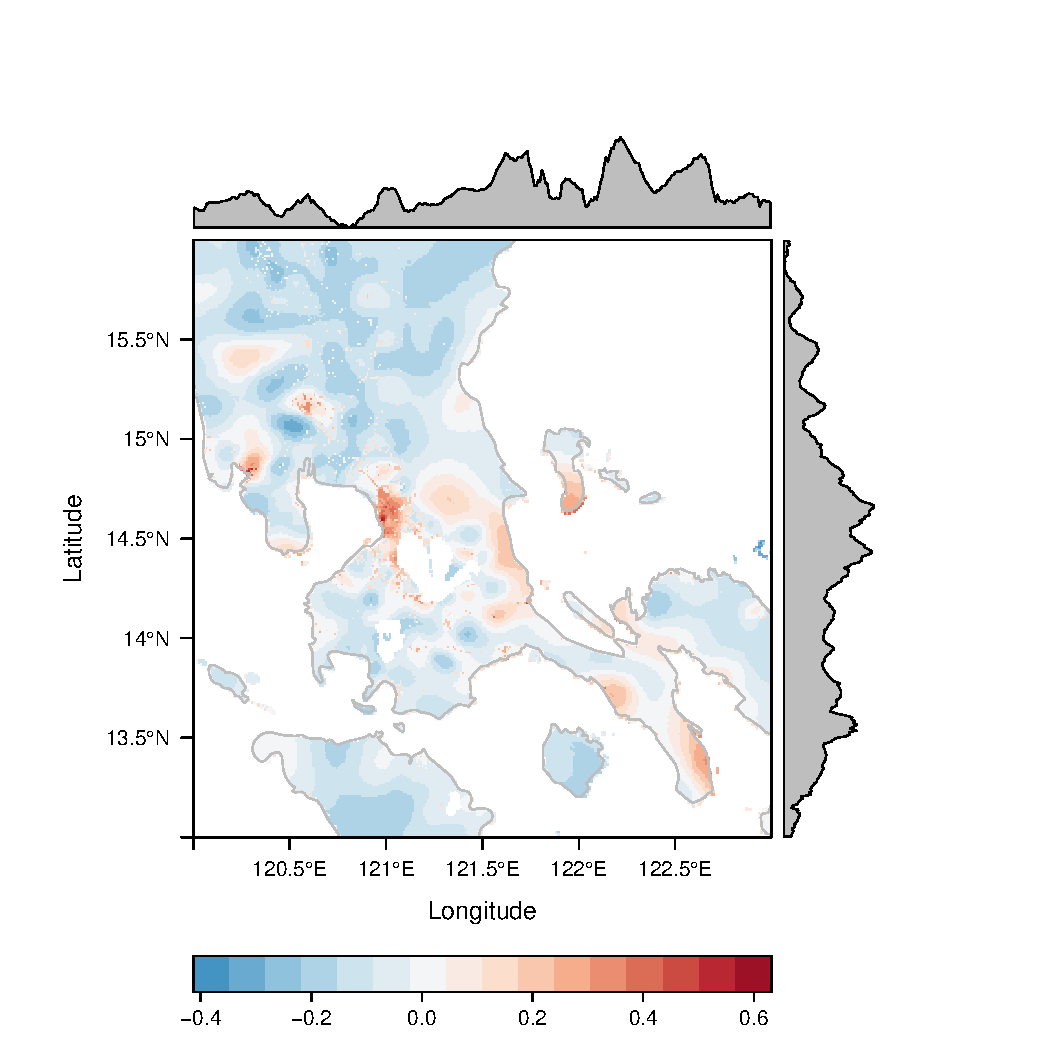
\includegraphics[width=0.475\textwidth]{sviNCR.pdf}
  }
  \subfloat[\label{fig:varNCR}]{
    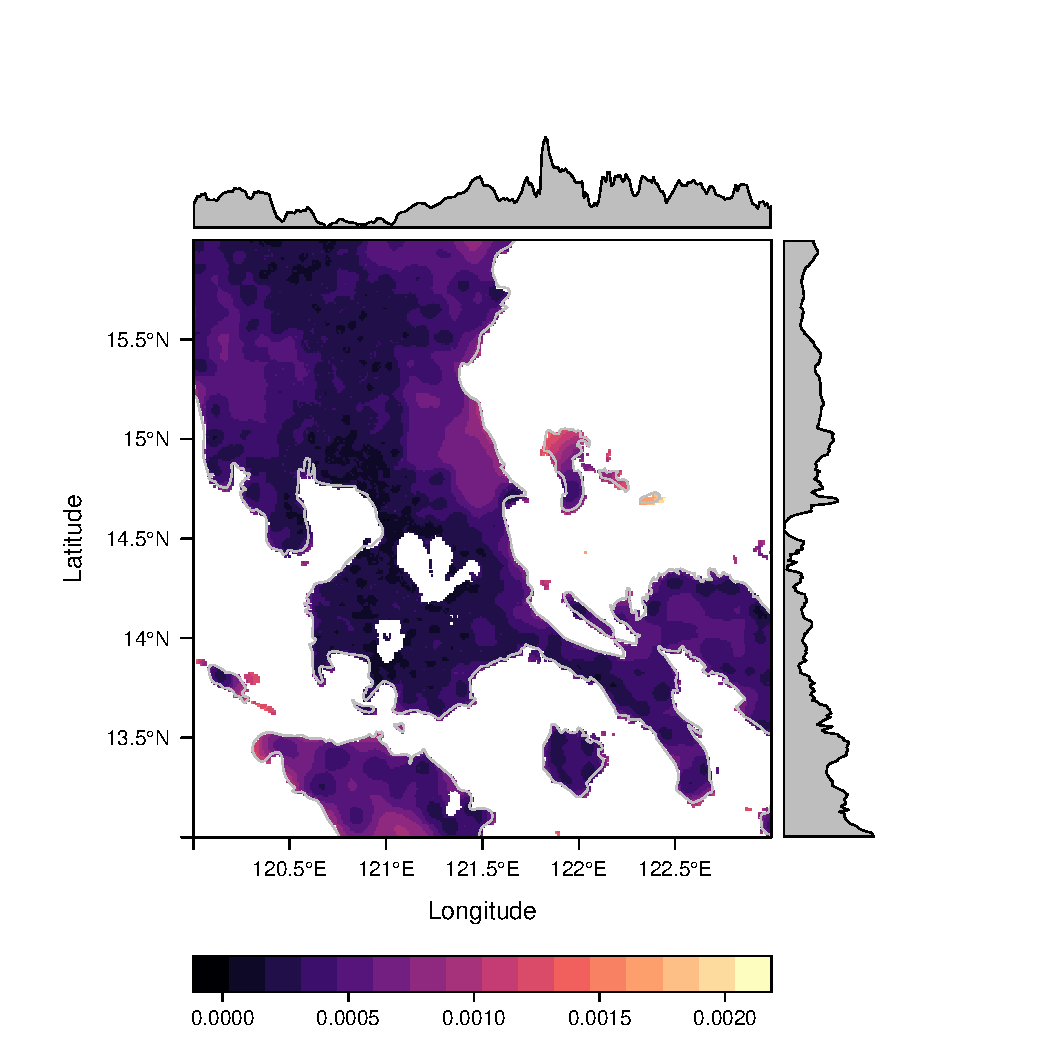
\includegraphics[width=0.475\textwidth]{var.pdf}
  }
  \caption{Social vulnerability (a) and prediction variance (b), National Capital Region, the Philippines, 1km scale}
\end{figure}

Figure~\ref{fig:svi} display the results of downscaling social vulnerability.  Associated with the model is interpolation uncertainty quantification, plotted around the National Capital Region, in figure~\ref{fig:varNCR}, this represents uncertainty due to the sizes of the input polygons; larger polygons and those further from other polygons have greater interpolation uncertainty--notice that islands and areas associated with Central Luzon--where administrative divisions encompass larger area--have higher uncertainty.  The plot margins are the row and column means of the plotted values--these can help highlight isolated and outlying areas that viewers might miss, for example the spots of high vulnerability in Palawan and Muslim Mindinao.

Interpolation uncertainty might help with decision making, but ultimately model results are based upon assumptions not testable within the framework of the model.  If we had the information necessary to assess the accuracy, we wouldn't need to solve the COSP in the first place.  The map in figure~\ref{fig:svi} is a {\em best linear unbiased prediction} (BLUP) based upon our knowledge of how spatial features may correlate or even cause social vulnerability; by {\em best} we mean no linear function exists able to achieve better prediction error.  We can improve upon it with focused research that tests and establishes relationships between social vulnerability and geographic space, and using data sets with wide geographic coverage to expand the applicability of resulting models to broader, hopefully global, ranges.

If one is comfortable with the assumptions of RK, it can be extrapolated via UK to locations beyond the area where the model was fit.  First use KED to fit a RK model and retain the $\bm{\beta}$ estimates.  Next supply these estimates to a UK model targeting the new area, which will use them to predict SVI before calculating residuals and kriging these values via SK with available georeferenced data.  This technique raises ethical and technical concerns that will require more room for discussion than is available now, however the final paragraphs of the section will touch upon these interesting aspects for future research.

The technical concern is that of extrapolation.  UK begins with an RWDM or KED model fit to data from a source geographic location, ideally where the data is less aggregated than at a target location where the model will be applied.  Looking again at equation~\ref{eq:rk}, we see that the calculated residuals will be the observed $\bm{y}$ values, from whatever level of aggregation, subtracted from the predicted value at the target resolution: $\bm{x}(s_i)^T \bm{\beta} - y(s_i)$.  Because these residuals are calculated from a model with greater geographic detail, they will share the same levels of geographic variability as the source model, and furthermore will assume the same relationship between the features of the source regression model and the dependent variable.  Thus, if some features have a different relationship in the source location, then the predictions of the model may be systematically biased.  Despite this additional level of detail in the residuals the kriging weights remain based upon the geographical aggregation of the dependent variable at the target location.  This means the details will be smoothed out by the size of the area to which the dependent variable is aggregated, and the uncertainty of the interpolated values will be greater.  In the event a sensible covariance function cannot be devised or fit to the data in the target location--e.g. if the data is georeferenced at too great a level of aggregation then the covariance function while have a large ``nugget'', or a variance in the measured value greater than zero as distance to the measurement approaches zero--then the SK step of UK will still fail or be unreliable.

Technical concerns of extrapolation are familiar, however these models are based on large, often government owned, data sets and may be burdened with subtle ethical if not legal questions.  Census data sets like those used to calculate and initially geolocate SVI are provided by foreign governments to non-nationals in goodwill for the purposes of research and education.  A model fit to that data, however, no longer needs the original data.  It can be applied with known error in the original location, or applied to any location with necessary input data, as long as one is willing to stomach the assumptions.  The model is based upon data provided for research, but the model could now be used sans the original data.  In this case, the concern is not one of privacy, confidentiality, or anonymity of persons in the data, but instead one of intent for how their data should be used.  Census data, like health data, represent personal information.  Privacy of citizens is already recognized as a concern for nations releasing their data through IPUMS-International \citep{mccaa06} and likewise researchers need also to consider issues that could arise when using this personal information to do things that go beyond the communities where it was collected.


\section{Conclusion}

This article has discussed the COSP as it concerns social sciences.  Solutions to the COSP allow social scientist to improve visualization of mapped data, combine data from unequal supports, or make estimates at supports other than where the data was collected.  The general solution to COSP is kriging: a flexible and robust spatial interpolation model that can be used for downscaling, upscaling, or sidescaling.  The article presented RWDM and RK for models that are suited to the needs of social science.  Both models allow ancillary georeferenced data to be used as predictors.  The key feature that distinguishes kriging models for population data from other kriging methods is the A2A/P covariance function that calculates covariance between two polygons or a polygon and point as the average covariance of points that discretize the polygons.

The article presented a spatial model of social vulnerability in the Philippines, and advised of potential technical and ethical concerns.  The model, fit in the Philippines, can be applied beyond that country's borders.  The Filipino census uses a geographically detailed sampling scheme that provides census data with high geographical resolution.  The high resolution provides a lot of information for the model fitting function to find associations between ancillary data and the variables under study; other areas of the world often lack this geographically detailed demographic information, especially in the areas of the world were we often would like to better understand social vulnerability.

The goal of this article was to present results of research into methods for downscaling population data to smaller supports, and to do so in a way that we hope encourage other social scientists to make broader use of these methods.  COSP solutions are varied: geographers typically wish to summarize data over larger levels of aggregation--the opposite goal of most social scientists.  Nonetheless, many of the solutions are useful for social science needs; the article discussed RWDM and RK with A2A/P covariance functions as particularly relevant for social scientists.  The methods can shed new light on spatial relationships and assist with spatial reasoning.  As social scientists apply these methods, however, they must remain aware that these methods can complicate existing concerns of privacy and usage of personal data collected in census and surveys.

\bibliography{bootstrap,boundary_detection,dasymetric,datasets,disasters,dissertation,gis,kriging,microsimulation,pop_topo,regression_modeling}

\end{document}
%%% Local Variables:
%%% mode: latex
%%% TeX-master: t
%%% End:
